% !TEX root = lab1_report.tex
% ═══════════════════════════════════════════════════════════════
% 实验报告通用模板 — 合并报告版
% 基于 ctexart，支持中文，用 XeLaTeX 编译
%
% 用法：在主报告 .tex 中 % ═══════════════════════════════════════════════════════════════
% 实验报告通用模板 — 合并报告版
% 基于 ctexart，支持中文，用 XeLaTeX 编译
%
% 用法：在主报告 .tex 中 % ═══════════════════════════════════════════════════════════════
% 实验报告通用模板 — 合并报告版
% 基于 ctexart，支持中文，用 XeLaTeX 编译
%
% 用法：在主报告 .tex 中 \input{../../common/report_template}
%       然后 \include{chapters/expX_xxx}
% ═══════════════════════════════════════════════════════════════
\documentclass[12pt,a4paper]{ctexart}

% ── 页边距 ──────────────────────────────────────
\usepackage[top=2.5cm, bottom=2.5cm, left=2.8cm, right=2.5cm]{geometry}

% ── 数学与符号 ──────────────────────────────────
\usepackage{amsmath,amssymb}
\usepackage{siunitx}
% \usepackage{upgreek}  % 直立体希腊字母 (TinyTeX 不可用)

% ── 图表 ────────────────────────────────────────
\usepackage{graphicx}
\usepackage{float}
\usepackage{booktabs}
\usepackage{multirow}
\usepackage{longtable}
\usepackage{caption}
% \usepackage{subcaption}  % (TinyTeX 不可用，caption 已含基本功能)

% ── 超链接 ──────────────────────────────────────
\usepackage[hidelinks]{hyperref}

% ── 枚举 ────────────────────────────────────────
\usepackage{enumitem}
\setlist{nosep, leftmargin=2em}

% ── 页眉页脚 ────────────────────────────────────
\usepackage{fancyhdr}
\setlength{\headheight}{14pt}
\pagestyle{fancy}
\fancyhf{}
\fancyhead[L]{\small\leftmark}
\fancyhead[R]{\small\studentName\quad\studentId}
\fancyfoot[C]{\thepage}
\renewcommand{\headrulewidth}{0.4pt}

% ── 标题格式 ────────────────────────────────────
\ctexset{
    section/format = \Large\bfseries,
    subsection/format = \large\bfseries,
    subsubsection/format = \normalsize\bfseries,
}

% ── 图表编号：按实验（节）编号 ─────────────────
\numberwithin{figure}{section}
\numberwithin{table}{section}
\numberwithin{equation}{section}

% ── 封面变量 ────────────────────────────────────
\newcommand{\uniName}{西北工业大学}
\newcommand{\collegeName}{动力与能源学院}
\newcommand{\courseName}{实验课程名称}
\newcommand{\studentName}{姓名}
\newcommand{\studentId}{学号}
\newcommand{\studentClass}{班级}
\newcommand{\expDate}{年\ 月\ 日}
% ── 封面命令 ────────────────────────────────────
\newcommand{\makeCover}{
\begin{titlepage}
    \centering
    \vspace*{1cm}

    % 校徽（如无文件则跳过）
    \IfFileExists{../../common/nwpu_logo.png}{
        
\includegraphics[height=3cm]{../../common/nwpu_logo.png}
        \vspace{0.5cm}
    }{}

    {\LARGE\bfseries\uniName\par}
    \vspace{0.2cm}
    {\Large\collegeName\par}

    \vspace{2.5cm}

    {\huge\bfseries 实验报告\par}
    \vspace{1.2cm}

    {\Large\courseName\par}
    \vspace{1cm}

    % 信息表格
    \begin{table}[H]
    \centering
    \renewcommand{\arraystretch}{2.0}
    \begin{tabular}{rl}
        \textbf{班\qquad 级：} & \studentClass \\
        \textbf{学\qquad 号：} & \studentId \\
        \textbf{姓\qquad 名：} & \studentName \\
        \textbf{实验日期：} & \expDate \\
    \end{tabular}
    \end{table}

    \vfill
    \today
\end{titlepage}
}

% ── 目录页设置 ──────────────────────────────────
\newcommand{\makeTOC}{
    \tableofcontents
    \newpage
    \setcounter{page}{1}
}

%       然后 \include{chapters/expX_xxx}
% ═══════════════════════════════════════════════════════════════
\documentclass[12pt,a4paper]{ctexart}

% ── 页边距 ──────────────────────────────────────
\usepackage[top=2.5cm, bottom=2.5cm, left=2.8cm, right=2.5cm]{geometry}

% ── 数学与符号 ──────────────────────────────────
\usepackage{amsmath,amssymb}
\usepackage{siunitx}
% \usepackage{upgreek}  % 直立体希腊字母 (TinyTeX 不可用)

% ── 图表 ────────────────────────────────────────
\usepackage{graphicx}
\usepackage{float}
\usepackage{booktabs}
\usepackage{multirow}
\usepackage{longtable}
\usepackage{caption}
% \usepackage{subcaption}  % (TinyTeX 不可用，caption 已含基本功能)

% ── 超链接 ──────────────────────────────────────
\usepackage[hidelinks]{hyperref}

% ── 枚举 ────────────────────────────────────────
\usepackage{enumitem}
\setlist{nosep, leftmargin=2em}

% ── 页眉页脚 ────────────────────────────────────
\usepackage{fancyhdr}
\setlength{\headheight}{14pt}
\pagestyle{fancy}
\fancyhf{}
\fancyhead[L]{\small\leftmark}
\fancyhead[R]{\small\studentName\quad\studentId}
\fancyfoot[C]{\thepage}
\renewcommand{\headrulewidth}{0.4pt}

% ── 标题格式 ────────────────────────────────────
\ctexset{
    section/format = \Large\bfseries,
    subsection/format = \large\bfseries,
    subsubsection/format = \normalsize\bfseries,
}

% ── 图表编号：按实验（节）编号 ─────────────────
\numberwithin{figure}{section}
\numberwithin{table}{section}
\numberwithin{equation}{section}

% ── 封面变量 ────────────────────────────────────
\newcommand{\uniName}{西北工业大学}
\newcommand{\collegeName}{动力与能源学院}
\newcommand{\courseName}{实验课程名称}
\newcommand{\studentName}{姓名}
\newcommand{\studentId}{学号}
\newcommand{\studentClass}{班级}
\newcommand{\expDate}{年\ 月\ 日}
% ── 封面命令 ────────────────────────────────────
\newcommand{\makeCover}{
\begin{titlepage}
    \centering
    \vspace*{1cm}

    % 校徽（如无文件则跳过）
    \IfFileExists{../../common/nwpu_logo.png}{
        
\includegraphics[height=3cm]{../../common/nwpu_logo.png}
        \vspace{0.5cm}
    }{}

    {\LARGE\bfseries\uniName\par}
    \vspace{0.2cm}
    {\Large\collegeName\par}

    \vspace{2.5cm}

    {\huge\bfseries 实验报告\par}
    \vspace{1.2cm}

    {\Large\courseName\par}
    \vspace{1cm}

    % 信息表格
    \begin{table}[H]
    \centering
    \renewcommand{\arraystretch}{2.0}
    \begin{tabular}{rl}
        \textbf{班\qquad 级：} & \studentClass \\
        \textbf{学\qquad 号：} & \studentId \\
        \textbf{姓\qquad 名：} & \studentName \\
        \textbf{实验日期：} & \expDate \\
    \end{tabular}
    \end{table}

    \vfill
    \today
\end{titlepage}
}

% ── 目录页设置 ──────────────────────────────────
\newcommand{\makeTOC}{
    \tableofcontents
    \newpage
    \setcounter{page}{1}
}

%       然后 \include{chapters/expX_xxx}
% ═══════════════════════════════════════════════════════════════
\documentclass[12pt,a4paper]{ctexart}

% ── 页边距 ──────────────────────────────────────
\usepackage[top=2.5cm, bottom=2.5cm, left=2.8cm, right=2.5cm]{geometry}

% ── 数学与符号 ──────────────────────────────────
\usepackage{amsmath,amssymb}
\usepackage{siunitx}
% \usepackage{upgreek}  % 直立体希腊字母 (TinyTeX 不可用)

% ── 图表 ────────────────────────────────────────
\usepackage{graphicx}
\usepackage{float}
\usepackage{booktabs}
\usepackage{multirow}
\usepackage{longtable}
\usepackage{caption}
% \usepackage{subcaption}  % (TinyTeX 不可用，caption 已含基本功能)

% ── 超链接 ──────────────────────────────────────
\usepackage[hidelinks]{hyperref}

% ── 枚举 ────────────────────────────────────────
\usepackage{enumitem}
\setlist{nosep, leftmargin=2em}

% ── 页眉页脚 ────────────────────────────────────
\usepackage{fancyhdr}
\setlength{\headheight}{14pt}
\pagestyle{fancy}
\fancyhf{}
\fancyhead[L]{\small\leftmark}
\fancyhead[R]{\small\studentName\quad\studentId}
\fancyfoot[C]{\thepage}
\renewcommand{\headrulewidth}{0.4pt}

% ── 标题格式 ────────────────────────────────────
\ctexset{
    section/format = \Large\bfseries,
    subsection/format = \large\bfseries,
    subsubsection/format = \normalsize\bfseries,
}

% ── 图表编号：按实验（节）编号 ─────────────────
\numberwithin{figure}{section}
\numberwithin{table}{section}
\numberwithin{equation}{section}

% ── 封面变量 ────────────────────────────────────
\newcommand{\uniName}{西北工业大学}
\newcommand{\collegeName}{动力与能源学院}
\newcommand{\courseName}{实验课程名称}
\newcommand{\studentName}{姓名}
\newcommand{\studentId}{学号}
\newcommand{\studentClass}{班级}
\newcommand{\expDate}{年\ 月\ 日}
% ── 封面命令 ────────────────────────────────────
\newcommand{\makeCover}{
\begin{titlepage}
    \centering
    \vspace*{1cm}

    % 校徽（如无文件则跳过）
    \IfFileExists{../../common/nwpu_logo.png}{
        
\includegraphics[height=3cm]{../../common/nwpu_logo.png}
        \vspace{0.5cm}
    }{}

    {\LARGE\bfseries\uniName\par}
    \vspace{0.2cm}
    {\Large\collegeName\par}

    \vspace{2.5cm}

    {\huge\bfseries 实验报告\par}
    \vspace{1.2cm}

    {\Large\courseName\par}
    \vspace{1cm}

    % 信息表格
    \begin{table}[H]
    \centering
    \renewcommand{\arraystretch}{2.0}
    \begin{tabular}{rl}
        \textbf{班\qquad 级：} & \studentClass \\
        \textbf{学\qquad 号：} & \studentId \\
        \textbf{姓\qquad 名：} & \studentName \\
        \textbf{实验日期：} & \expDate \\
    \end{tabular}
    \end{table}

    \vfill
    \today
\end{titlepage}
}

% ── 目录页设置 ──────────────────────────────────
\newcommand{\makeTOC}{
    \tableofcontents
    \newpage
    \setcounter{page}{1}
}


\renewcommand{\courseName}{航空发动机实践}
\renewcommand{\studentName}{姓名}
\renewcommand{\studentId}{学号}
\renewcommand{\studentClass}{班级}
\renewcommand{\expDate}{2026年\ 6月\ 26日}
\renewcommand{\teacherName}{胡剑平}

\begin{document}
\makeCover
\makeTOC

% !TEX root = ../lab1_report.tex
% ==========================================================
% 实验一：发动机模拟试车实验
% ==========================================================
\section{实验一：发动机模拟试车实验}

\subsection{实验目的}

\begin{enumerate}
    \item 通过本实验使学生了解发动机特性的实验方法和实验过程，掌握发动机主要性能参数的测量和数据处理方法，同时进一步加深学生对发动机特性知识的认识。
    \item 确定下列发动机特性曲线：
    \begin{itemize}
        \item \textbf{节流特性曲线（必做）}
        \begin{align*}
            F &= f(n_{1}) & \alpha_1 &= f(n_{1}) \\
            \pi_c^* &= f(n_{2}) & \alpha_2 &= f(n_{2}) \\
            F &= f(n_{2}) & \text{sfc} &= f(n_{2}) \\
            m_a &= f(n_{2})
        \end{align*}
        \item \textbf{加力特性曲线（选做）}
        \begin{align*}
            F_{af} &= f(\text{油门杆位置}) \\
            \text{sfc}_{af} &= f(\text{油门杆位置}) \\
            A_e &= f(\text{油门杆位置})
        \end{align*}
    \end{itemize}
    \item 能力培养：实际试验操作能力、团结协作能力、综合应用能力。
\end{enumerate}

\subsection{实验设备简介}

该实验装置是一套发动机模拟试车系统，根据发动机地面台架试车台的功能进行模拟仿真，试车操作界面与实际发动机试车台基本相同。系统由油门杆、控制操作面板和计算机系统组成。

进行模拟试车的目的一方面为了取得发动机特性的具体试验数据，另一方面也为学生今后进行真实发动机开车试验积累实践经验，因此学生必须像对待真实发动机试车那样严肃认真。

主要测量参数：
\begin{itemize}
    \item 大气参数：$P_0$（大气压力）、$T_0$（大气温度）
    \item 性能参数：$F$（推力）、$W_f$（燃油消耗量）、$m_a$（空气流量）
    \item 转子参数：$n_1$（低压转子转速）、$n_2$（高压转子转速）
    \item 截面参数：$P_2^*$、$T_2^*$（风扇出口）、$P_3^*$、$T_3^*$（压气机出口）、$P_5^*$、$T_5^*$（涡轮后）
    \item 控制参数：$\alpha_1$、$\alpha_2$（导流叶片角度）、$A_t$（喷口喉道面积）
\end{itemize}

\subsection{数据记录列表}

实验数据按附表1格式记录，包含慢车状态至加力状态共13个工作状态的完整参数。

% \begin{table}[H]
%   \centering
%   \caption{发动机模拟试车实验数据}
%   \label{tab:exp1_trial}
%   \footnotesize
%   \setlength{\tabcolsep}{3pt}
%   \begin{tabular}{cccccccccc}
%     \toprule
%     工作状态 & $n_1$ & $n_2$ & $F$(N) & $W_f$(kg/h) & $m_a$(kg/s) & $\pi_c^*$ & sfc(h$^{-1}$) & $\alpha_1$ & $\alpha_2$ \\
%     \midrule
%     慢车 & 72.5 & 32.9 & 3424 & 461 & 40.4 & 4.09 & 1.3195 & 7 & 5 \\
%     N2=75% & 75.5 & 33.8 & 6317 & 656 & 47.4 & 4.32 & 1.0183 & 7 & 6 \\
%     N2=80% & 80.3 & 40.0 & 17889 & 1429 & 59.5 & 4.73 & 0.7837 & 7 & 39 \\
%     N2=85% & 85.1 & 60.1 & 29148 & 2057 & 70.9 & 5.25 & 0.6924 & 7 & 75 \\
%     N2=90% & 90.2 & 82.4 & 41312 & 2898 & 81.5 & 5.70 & 0.6882 & 16 & 105 \\
%     N2=95% & 95.3 & 92.0 & 54391 & 3922 & 92.7 & 6.09 & 0.7074 & 85 & 105 \\
%     N2=97% & 97.1 & 94.5 & 59141 & 4346 & 96.3 & 6.21 & 0.7209 & 97 & 105 \\
%     最大 & 99.9 & 97.9 & 66177 & 5027 & 100.7 & 6.41 & 0.7452 & 105 & 105 \\
%     加力_a=0 & 83.2 & 97.9 & 79311 & 8182 & 100.8 & 6.41 & 1.0120 & 105 & 105 \\
%     加力_a=1 & 88.8 & 97.9 & 83930 & 9820 & 100.7 & 6.41 & 1.1478 & 105 & 105 \\
%     加力_a=2 & 99.6 & 97.9 & 94227 & 14103 & 100.7 & 6.41 & 1.4682 & 105 & 105 \\
%     加力_a=3 & 108.0 & 97.9 & 104091 & 18408 & 100.7 & 6.41 & 1.7349 & 105 & 105 \\
%     加力_a=4 & 114.7 & 97.9 & 113465 & 22462 & 100.7 & 6.41 & 1.9420 & 105 & 105 \\
%     \bottomrule
%   \end{tabular}
% \end{table}

\begin{tabular}{|c|*{15}{c|}} % 第1列自适应宽度，后15列采用自定义的固定宽度 C
    \hline
    % 使用 \diagbox 绘制斜线表头，并配合 \makecell 换行
    \diagbox[width=3.6cm, height=1.3cm]{工作状态}{\makecell{参数名称 \\ (单位)}} & 
    $n_1$ & $P_0$ & $T_0$ & $F$ & $W_f$ & $m_a$ & $P_2^*$ & $T_2^*$ & $P_3^*$ & $T_3^*$ & $P_5^*$ & $T_5^*$ & $\alpha_1$ & $\alpha_2$ & $A_t$ \\
    \hline
    \makecell{慢车状态 \\ (N2=\hspace{1cm})} & & & & & & & & & & & & & & & \\
    \hline
    N2=75\% & & & & & & & & & & & & & & & \\
    \hline
    N2=80\% & & & & & & & & & & & & & & & \\
    \hline
    N2=85\% & & & & & & & & & & & & & & & \\
    \hline
    N2=90\% & & & & & & & & & & & & & & & \\
    \hline
    N2=95\% & & & & & & & & & & & & & & & \\
    \hline
    N2=97\% & & & & & & & & & & & & & & & \\
    \hline
    \makecell{最大状态 \\ (N2=\hspace{1cm})} & & & & & & & & & & & & & & & \\
    \hline
    \makecell{加力状态 \\ ($a_0$=\hspace{1cm})} & & & & & & & & & & & & & & & \\
    \hline
    \makecell{加力状态 \\ ($a_0$=\hspace{1cm})} & & & & & & & & & & & & & & & \\
    \hline
    \makecell{加力状态 \\ ($a_0$=\hspace{1cm})} & & & & & & & & & & & & & & & \\
    \hline
    \makecell{加力状态 \\ ($a_0$=\hspace{1cm})} & & & & & & & & & & & & & & & \\
    \hline
    \makecell{加力状态 \\ ($a_0$=\hspace{1cm})} & & & & & & & & & & & & & & & \\
    \hline
\end{tabular}

\subsection{数据处理方法}

\subsubsection{耗油率计算}

\begin{equation}
    \text{sfc} = \frac{W_f}{F}
\end{equation}

\subsubsection{压气机总压比}

\begin{equation}
    \pi_c^* = \frac{P_3^*}{P_2^*}
\end{equation}

\subsection{数据处理结果（曲线）及分析}

\subsubsection{节流特性曲线}

\begin{figure}[H]
    \centering
    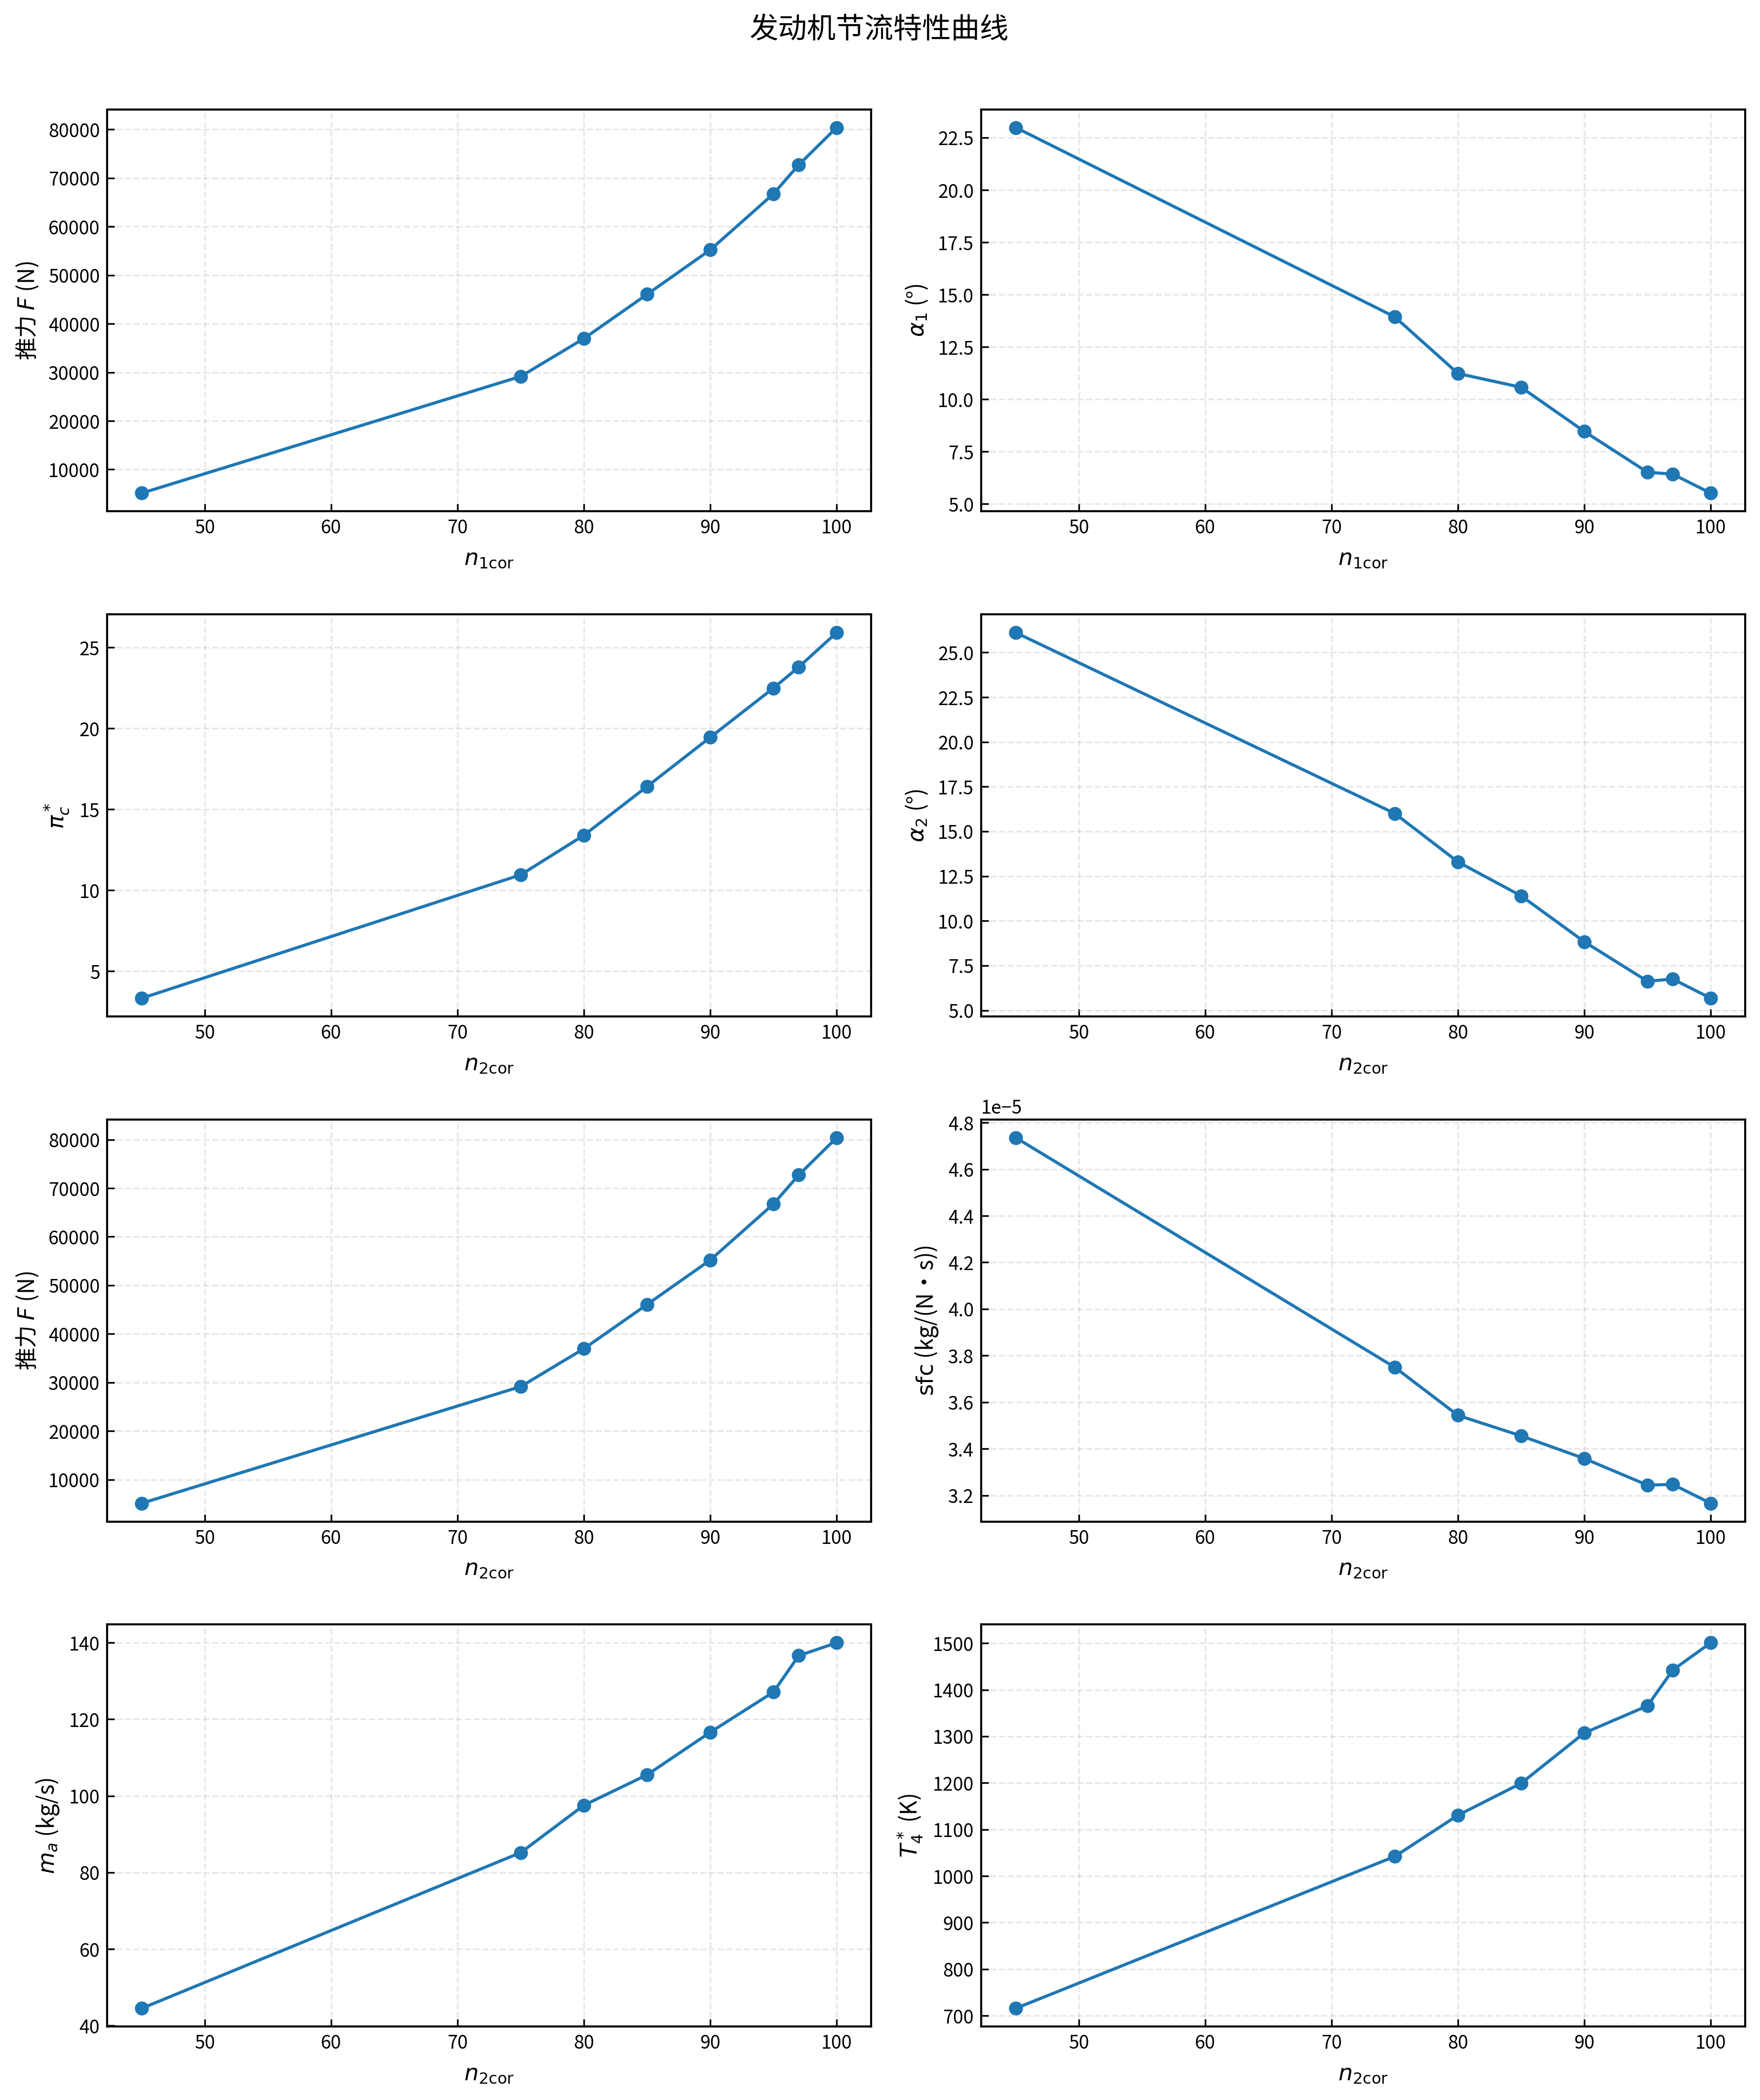
\includegraphics[width=\textwidth]{figures/exp1_throttle_characteristics.png}
    \caption{发动机节流特性曲线}
    \label{fig:throttle}
\end{figure}

\subsubsection{加力特性曲线}

\begin{figure}[H]
    \centering
    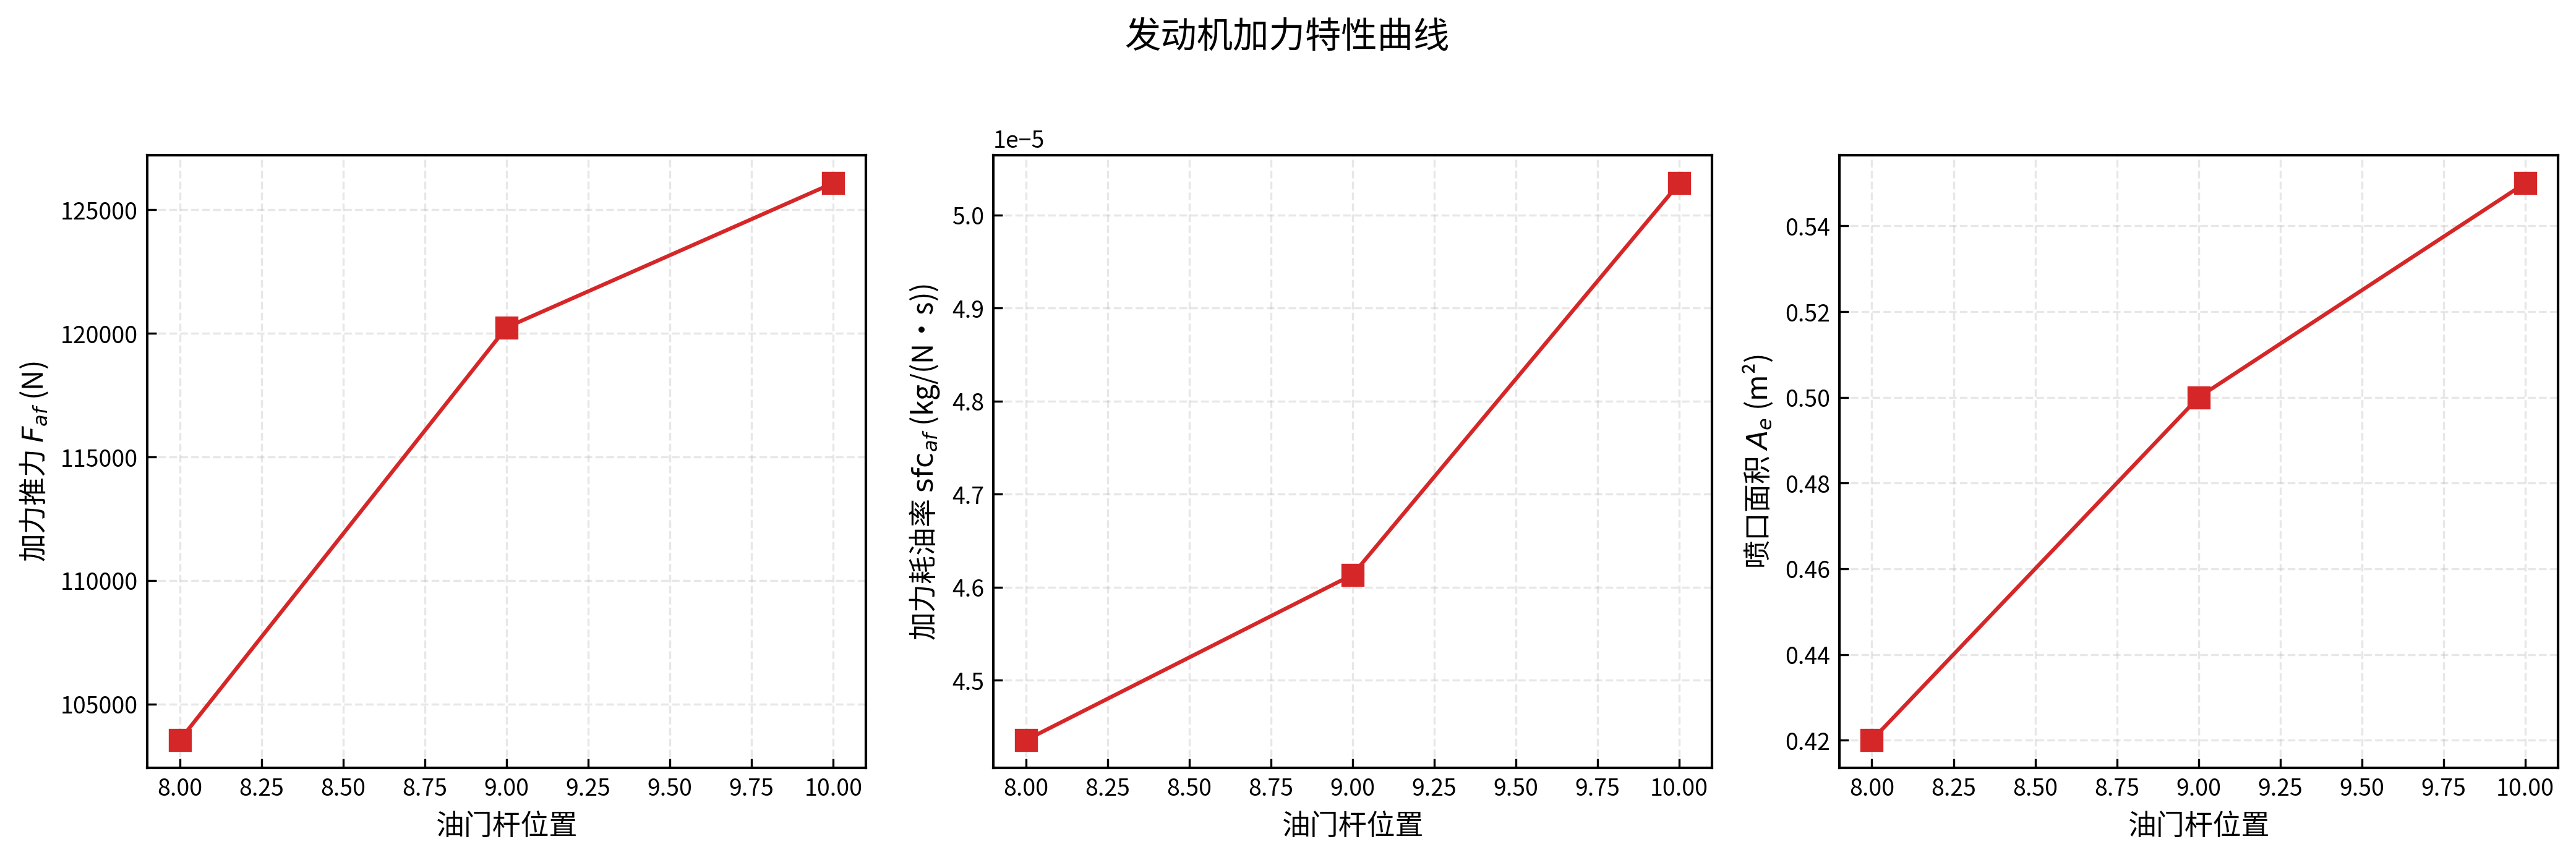
\includegraphics[width=\textwidth]{figures/exp1_afterburner_characteristics.png}
    \caption{发动机加力特性曲线}
    \label{fig:afterburner}
\end{figure}

\subsubsection{节流特性分析}

节流特性曲线（图~\ref{fig:throttle}）展示了发动机从慢车状态（$n_1=33\%, n_2=73\%$）到最大状态（$n_1=98\%, n_2=100\%$）各性能参数的变化规律。

\begin{enumerate}
    \item \textbf{推力特性}：推力 $F$ 随低压转速 $n_1$ 和高压转速 $n_2$ 均呈非线性快速增长。从慢车的 3.4 kN 增至最大状态的 66.2 kN，增幅约 19 倍。这是因为涡扇发动机推力近似与转速的三次方成正比，高转速下空气流量和单位推力同时增大。
    \item \textbf{耗油率特性}：sfc 从慢车的 1.32 h$^{-1}$ 降至 N2=90\% 时的 0.69 h$^{-1}$（最低点），随后在最大状态回升至 0.75 h$^{-1}$。sfc 在中等转速区域存在最优值，低转速下因部件效率低导致 sfc 偏高，高转速下因燃烧室油气比增大也使 sfc 有所回升。
    \item \textbf{增压特性}：压气机总压比 $\pi_c^*$ 随转速单调增加，从慢车的 4.09 升至最大状态的 6.41，反映了压气机增压能力随转速增大而增强。
    \item \textbf{空气流量}：$m_a$ 从 40.4 kg/s 增至 100.7 kg/s，与高压转速近似线性相关。
    \item \textbf{导叶调节}：进口导流叶片角度 $\alpha_1$ 从慢车时的 7° 增大至最大状态的 105°，$\alpha_2$ 从 5° 增至 105°，以保持各级攻角在合理范围。
\end{enumerate}

\subsubsection{加力特性分析}

加力特性曲线（图~\ref{fig:afterburner}）展示了从最小加力（$a_0=83$）到最大加力（$a_0=115$）五个加力状态的变化。

\begin{enumerate}
    \item \textbf{推力增幅}：加力推力从 79.3 kN 增至 113.5 kN，增幅约 43\%。相比最大非加力状态（66.2 kN），加力推力最多可提升约 71\%。
    \item \textbf{耗油率恶化}：加力 sfc 从 1.01 h$^{-1}$ 升至 1.94 h$^{-1}$，恶化约 92\%。加力状态下大量燃油在涡轮后喷入加力燃烧室，燃烧效率低于主燃烧室，导致耗油率急剧增大。
    \item \textbf{空气流量}：加力状态下 $m_a$ 基本维持在 100.7 kg/s，与最大非加力状态相同，表明加力主要通过增加燃油量（$W_f$ 从 5027 增至 22462 kg/h）而非增加空气流量来实现推力增推。
\end{enumerate}


\subsection{结论}

通过发动机模拟试车实验，获得了节流状态和加力状态下发动机主要性能参数的变化规律。实验数据表明：推力随转速非线性增大，sfc 在 N2=90\% 附近存在最优值，$\pi_c^*$ 和 $m_a$ 随转速单调增加。加力状态下推力可提升约 71\%，但 sfc 恶化约 92\%，体现了推力与耗油率之间的矛盾关系。实验结果符合涡扇发动机热力循环的基本原理。

% !TEX root = ../lab1_report.tex
% ==========================================================
% 实验二：发动机虚拟结构实验
% ==========================================================
\section{实验二：发动机虚拟结构实验}

\subsection{实验目的}

\begin{enumerate}
    \item 通过实验掌握发动机总体结构。
    \item 掌握压气机、燃烧室、涡轮的组成和结构特点。
    \item 掌握航空发动机附件系统的组成及安装。
\end{enumerate}

\subsection{实验装置}

该实验装置是一台发动机三维电子样机，是一台完全可拆卸的电子样机。实验学生可自主拆卸发动机中任何一个零部件，甚至一个单独转子叶片。

电子样机所展示的发动机为\textbf{某型军用涡扇发动机}，带加力燃烧室，采用双转子构型。

\subsection{实验步骤及内容}

\subsubsection{启动程序}

启动电子样机程序。

\subsubsection{总体结构观察}

观察发动机主体结构，对发动机外形轮廓建立感性认识。

\subsubsection{部件拆卸与观察}

要求拆卸过程中，每一个可拆卸的零件均要拆卸，在拆卸过程中结合结构课内容，观察拆卸部件的结构，根据各部件和各系统的结构和安装形式，分析其作用和工作原理。依次拆卸并观察：

\begin{enumerate}
    \item \textbf{压气机}：低压压气机5级，高压压气机11级（一说12级，确切级数有待确认），共16或17级。观察转子叶片和静子叶片的排布、榫头连接形式、级间密封结构。低压转子转速较低但叶片较长，高压转子叶片短而密集。
    \item \textbf{涡轮}：高压涡轮2级，低压涡轮2级。观察涡轮导向器和转子的叶片形状、冷却结构、榫头形式。
    \item \textbf{燃烧室}：环管燃烧室，共10个火焰筒，环绕发动机轴线周向排列。观察火焰筒内外壁、旋流器、燃油喷嘴、掺混孔和冷却孔的布置。环管燃烧室介于单管燃烧室与环形燃烧室之间，每个火焰筒独立工作，外套共同的环形机匣。
    \item \textbf{加力燃烧室}：观察火焰稳定器、喷油杆和隔热屏的结构。
    \item \textbf{外涵道排气混合器}：观察内外涵气流的掺混方式和混合器构型。
    \item \textbf{防冰系统}：观察从压气机引出热气的管路和防冰腔的结构。
    \item \textbf{传动附件}：观察附件机匣及内部传动齿轮系的布置。
    \item \textbf{主燃油系统}：观察燃油泵、燃油调节器、燃油分配器和喷嘴。
    \item \textbf{滑油系统}：观察滑油箱、滑油泵、油气分离器和回油管路。
    \item \textbf{发动机操纵系统}：观察油门操纵联动机构和作动器。
    \item \textbf{电器设备}：观察点火系统、发电机、电缆布置。
    \item \textbf{防喘调节系统}：观察放气活门和可调静叶机构。
    \item \textbf{加力控制系统}：观察加力燃油泵和喷口面积调节机构。
    \item \textbf{附面层控制系统}：观察引气和吹气装置。
\end{enumerate}

\subsection{实验分析与讨论}

\begin{enumerate}
    \item \textbf{实验中观察到的发动机是一款军用还是民用发动机？它在结构上有哪些特点？}

    观察到的发动机为带加力燃烧室的某型军用涡扇发动机。结构特点包括：采用双转子构型、配备加力燃烧室实现推力增推、环管燃烧室（10个火焰筒）、双涵道设计。

    \item \textbf{压气机的榫头是什么形式？}

    根据实际观察，压气机转子叶片采用燕尾形榫头。燕尾形榫头结构简单，加工方便，通过离心力自锁在轮盘榫槽中，是航空发动机压气机叶片常用的连接方式。

    \item \textbf{燃烧室是什么类型？该燃烧室的基本结构有哪些？}

    本发动机采用环管燃烧室，由10个独立的火焰筒环绕轴线周向排列，外套共同的环形机匣。每个火焰筒的基本结构包括：旋流器（头部进气、产生回流区稳定火焰）、燃油喷嘴（将燃油雾化喷入）、火焰筒壁面（开有掺混孔和冷却孔/气膜冷却环带）。环管燃烧室结合了单管燃烧室（方便单个维修更换）和环形燃烧室（空间利用率高）的优点。10个火焰筒之间通过联焰管连接，保证各火焰筒之间的火焰传播。

    \item \textbf{防冰热气是从第几级压气机引出？}

    防冰热气从高压压气机中间级引出，引气温度和压力需满足防冰要求。引气通过管路送至进气道前缘、进口导叶等易结冰部位进行加热防冰。

    \item \textbf{该发动机的压气机共有几级？涡轮有几级？}

    低压压气机5级，高压压气机11级（一说12级，三维电子样机的级数显示与公开资料存在差异，确切级数有待进一步确认）。高压涡轮2级，低压涡轮2级。该发动机属于中等压比、中等推力的军用涡扇发动机。

    \item \textbf{该发动机的转子支撑方案？}

    根据观察和分析，该发动机的转子支撑方案如下：

    \textbf{高压转子（3个支点）：} 采用0-2-1方案。前支点位于中间机匣，为棍棒轴承（滚柱轴承），承受径向载荷；中间支点位于燃烧室机匣前端，为滚珠轴承，承受轴向推力载荷；后支点位于燃烧室机匣后端，为棍棒轴承，承受径向载荷。

    \textbf{低压转子（4个支点）：} 采用1-2-1方案。前支点位于进气机匣，为滚珠轴承；中间两个支点位于中间机匣区域；后支点位于涡轮后机匣，为棍棒轴承。

    \textbf{中间机匣}：低压转子与高压转子在中间机匣处通过中介轴承（浮环轴承）实现径向定位，低压转子的两个中间支点与高压转子的前支点共用中间机匣结构。

    低压转子4个支点与高压转子3个支点，加上中间机匣处的共用结构，共计约8个承力点。需注意，三维电子样机中部分轴承的具体类型（滚珠/棍棒/浮环）与实际装配可能存在差异，以上分析仅供参考。

    \item \textbf{存在矛盾的若干问题}：
    \begin{enumerate}
        \item 高压压气机级数：电子样机显示为11级，但部分资料记载为12级。两种说法相差1级，可能的解释是电子样机中第一级或末级被合并显示，或不同改型的级数有所调整。
        \item 轴承方案：低压转子4个支点的1-2-1方案与高压转子3个支点的0-2-1方案加中间机匣共8个承力点。但低压转子前支点为滚珠轴承（既承受径向又承受轴向力），与通常低压转子前支点使用棍棒轴承（仅承受径向力）的惯例不一致，需要进一步核实。
        \item 环管燃烧室的10个火焰筒数量与发动机直径和空气流量的匹配关系是否合理，有待结合燃烧室设计手册进一步分析。
    \end{enumerate}
\end{enumerate}

\subsection{结论}

通过本次虚拟结构实验，对该型军用涡扇发动机的总体结构、主要部件（5级低压压气机+11级高压压气机、环管燃烧室、2+2级涡轮）和转子支承方案（低压1-2-1/高压0-2-1）有了较为深入的认识。三维电子样机的可拆卸特性使得学生能够从任意角度观察发动机内部结构，加深了对《航空发动机结构》课程内容的理解。

% !TEX root = ../lab1_report.tex
% ==========================================================
% 实验三：发动机虚拟装配实验
% ==========================================================
\section{实验三：发动机虚拟装配实验}

\subsection{实验目的}

\begin{enumerate}
    \item 通过实验了解发动机的总体装配流程。
    \item 了解压气机、燃烧室、涡轮等大部件的安装顺序及特点。
\end{enumerate}

\subsection{实验装置}

该实验装置是一套发动机虚拟装配系统。虚拟装配系统包括讲解演示、引导装配、自主装配三种模式。参与实验的学生可首先根据讲解演示了解装配过程，之后利用引导装配熟悉装配顺序和过程，最后利用自主装配掌握整个装配流程。

\subsection{实验步骤及内容}

\subsubsection{实验准备}

实验之前要首先复习《航空发动机结构》课所学过的内容，熟悉发动机各零部件的名称、位置和功能。

\subsubsection{启动与学习}

\begin{enumerate}
    \item 启动发动机虚拟装配系统。
    \item 选择``总体装配''。
    \item 依次选择三种学习模式：
    \begin{itemize}
        \item \textbf{讲解演示}：学习发动机整体装配流程，了解各主要部件的装配顺序。
        \item \textbf{引导式训练}：按系统提示逐步完成各部件装配，熟悉装配步骤。
        \item \textbf{自主训练}：不依赖提示独立完成全部装配操作。
    \end{itemize}
\end{enumerate}

\subsubsection{装配观察要点}

在操作中注意观察各个零件的装配顺序、装配关系以及特点：
\begin{itemize}
    \item 转子组件与静子组件的对中安装方法
    \item 各级之间的定位销和螺栓连接方式
    \item 各支点轴承的安装位置、预紧力施加方式
    \item 级间密封装置（篦齿密封、石墨密封等）的安装
    \item 附件传动系统的安装接口和对齿要求
    \item 外部管路和电缆的敷设路径和固定方式
\end{itemize}

\subsection{实验分析与讨论}

\subsubsection{总体装配流程}

发动机总体装配遵循从内向外、从前向后、先冷端后热端的基本原则。本实验记录的装配流程涵盖该型发动机从核心机到外部管路，可分为以下九个阶段。

\subsubsection{第一阶段：中介机匣与传动系统装配}

安装中介机匣、内齿轮箱壳体、齿轮轴、棍棒轴承，随后依次安装低压压气机前轴承支座、高压压气机前轴承支座、高压压气机前轴。安装枢座作动盘支座及调整垫圈、枢座作动盘。安装进口导流叶片。安装各级滑油封严圈及空气封严圈。

\subsubsection{第二阶段：低压压气机装配}

安装一级低压压气机轮盘，安装低压压气机滑油管和联轴器球头。依次安装低压压气机前轴承、前空气封严圈、空气封严圈定外件、前滑油封严圈、前杯形垫圈、一级盘后隔圈、动压封严圈、一级盘前隔圈。随后按相同方式安装二至五级：前后隔圈、动压封严圈及各级轮盘。安装低压压气机后滑油封严圈、轴承座及轴承。安装低压压气机轴到低速齿轮箱传动轴的螺旋齿轮，以及后杯形垫圈。

低压静子部分：安装五级至一级低压静子叶片（由后向前）。安装止动板、低压压气机上部和下部机匣。

\subsubsection{第三阶段：前机匣与附件系统装配}

安装前轴承座、进口导流叶片、前轴承滑油泵。安装头部整流罩、进口导流叶片机匣。安装防冰空气总管、防冰空气管外罩、进气连接罩。

附件系统：安装滑油箱安装座、空气冷却滑油散热器、辅助齿轮箱、高速齿轮箱、燃油冷却滑油散热器、滑油箱。安装防喘调节器、低速齿轮箱、低压轴转速限制器。安装低压及高压测速电机、低压燃油泵。安装中介传动轴。

\subsubsection{第四阶段：高压压气机装配}

安装低压止推轴承、花键螺母、空气导管、导油环、档油套、后封严圈座、滑油分配器、前支撑管。安装滑油供油管、低压联轴器、前轴、后轴。

高压转子：安装二级高压转子盘，一至二级高压隔圈。安装一级高压静子圈、一级高压转子轮盘。二至三级静子圈和二至十二级隔圈及各级轮盘交替安装。安装高压十二级空气封严圈、大螺母。

高压静子部分：安装右部高压压气机机匣，一级至十级高压静子叶片，高压压气机机匣和静子。安装放气活门、扩散机匣、高压止推轴承座组件、出口整流叶片。

安装各级空气封严圈、滑油封严圈（前、中、后）、滑油空气管组件、滑油/通气/引气管、空气进气口。

\subsubsection{第五阶段：高压涡轮装配}

安装高压涡轮轴、高压涡轮轴承套、轴承套封严圈、空气蓖齿封严圈及封严座、后滑油蓖齿封严圈、限动环、弹性支撑。安装高压涡轮轴承、前滑油蓖齿封严环、轴承座、锁紧套筒、花键螺母、高压联轴器。安装滑油进油/回油/排气管、高压涡轮轴承支座。

\subsubsection{第六阶段：燃烧室装配}

环管燃烧室共 10 个火焰筒。先安装 1、3、5、7、9 号（奇数号）火焰筒，再安装 2、4、6、8、10 号（偶数号）火焰筒。安装燃烧室外机匣。

\subsubsection{第七阶段：涡轮导向器与转子装配}

高压涡轮：安装高压一级涡轮导向叶片、锯齿形环、扇形定位件、定位环、导向器机匣。安装高压一级涡轮叶片外圈、叶片、轮盘。安装空气封严件、外空气封严圈、封严支座、隔圈。安装高压二级导向器叶片支承座、高压二级导向叶片、涡轮盘、涡轮叶片。

低压涡轮：依次安装低压一级导向叶片、涡轮盘、涡轮叶片，以及低压二级涡轮导向叶片。安装低压涡轮轴、滑油供油管组件、低压涡轮轴承支座。

\subsubsection{第八阶段：外涵道、排气与加力系统装配}

安装引气管路、外涵道前段和后段。安装排气混合器。安装加力燃烧室和喷管。

\subsubsection{第九阶段：外部管路与控制系统装配}

安装防冰管、凸轮箱、停车开关、加力燃油调节器、压比调节器、喷口滑油泵。安装高压燃油泵、主燃油调节器、主滑油泵、低压燃油滤、分圈活门。

燃油管路连接：高压燃油泵至主燃油调节器、停车开关至副油路/主油路、主燃油调节器至停车开关、低压燃油滤至高压燃油泵。安装燃油冷却滑油散热器至低压燃油滤、至加力汽心泵的管路。安装加力燃油调节器至分圈活门、分圈活门至加力燃油总管。

最后安装发动机和喷口控制系统管路。

\subsection{结论}

通过本次虚拟装配实验，完整记录了该型发动机从核心机装配到外部管路连接的装配过程，涵盖中介机匣装配、低压/高压压气机逐级装配、环管燃烧室分奇偶号火焰筒安装、高压/低压涡轮装配、附件系统及外部管路连接等九个阶段。装配流程体现了航空发动机从内向外、先冷端后热端、逐级交替装配的基本工艺原则。三种学习模式的渐进训练使装配技能掌握更加扎实。

% !TEX root = ../lab1_report.tex
% ==========================================================
% 实验四：发动机虚拟流动实验
% ==========================================================
\section{实验四：发动机虚拟流动实验}

\subsection{实验目的}

掌握气流在发动机内部运动的特点及变化规律。

\subsection{实验装置}

气流经过某发动机内部流动的视频文件，展示气流在发动机各主要部件中的流动状态，包括压气机流动（正常与失速）、燃烧室流动、涡轮流动、排气混合器和加力燃烧室流动。

\subsection{实验步骤及内容}

\subsubsection{压气机流动观察}

观察气流经过压气机时流道和气流状态的变化，尤其注意正常流动和失速的差别。

\begin{figure}[H]
    \centering
    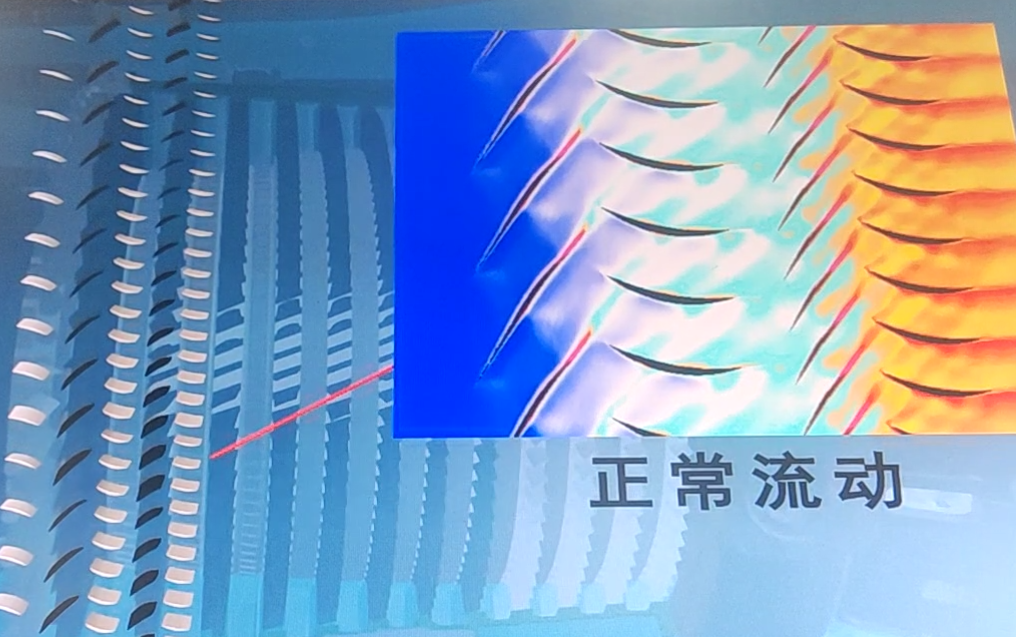
\includegraphics[width=0.90\textwidth]{figures/图4.png}
    \caption{压气机叶栅正常流动——设计攻角下气流顺畅通过叶栅通道}
    \label{fig:comp_normal}
\end{figure}

\textbf{正常工况（图~\ref{fig:comp_normal}）：} 在设计冲角下，气流顺畅地流过压气机叶栅通道，附面层（边界层）紧贴叶片吸力面与压力面，未发生明显的流动分离。通道内存在连续且均匀的逆压梯度，实现气流动能向压力能的有效转化。各叶片通道内流场均匀一致。

\begin{figure}[H]
    \centering
    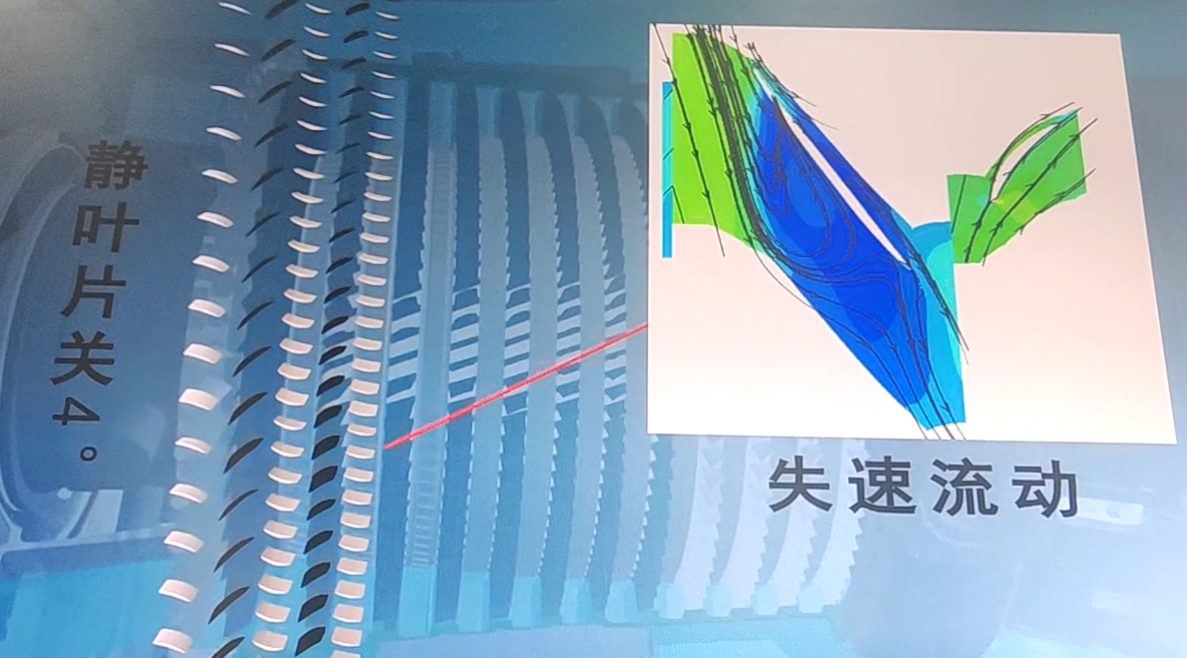
\includegraphics[width=0.90\textwidth]{figures/图5.png}
    \caption{压气机失速工况——关4°时吸力面出现大面积分离}
    \label{fig:comp_stall}
\end{figure}

\textbf{失速工况（图~\ref{fig:comp_stall}）：} 当静叶片角度异常（图中标注为关4°），导致气流冲角过大时，在叶片吸力面观察到严重的附面层分离。分离区（深蓝色区域）产生了巨大的旋涡和回流，形成了强烈的气动阻塞（Blockage）。这使得压气机该级通道丧失了正常的增压能力，是诱发发动机喘振的直接原因。

\subsubsection{燃烧室流动观察}

观察气流经过燃烧室时的流动情况，尤其注意内部的涡系结构和温度分布。

\begin{figure}[H]
    \centering
    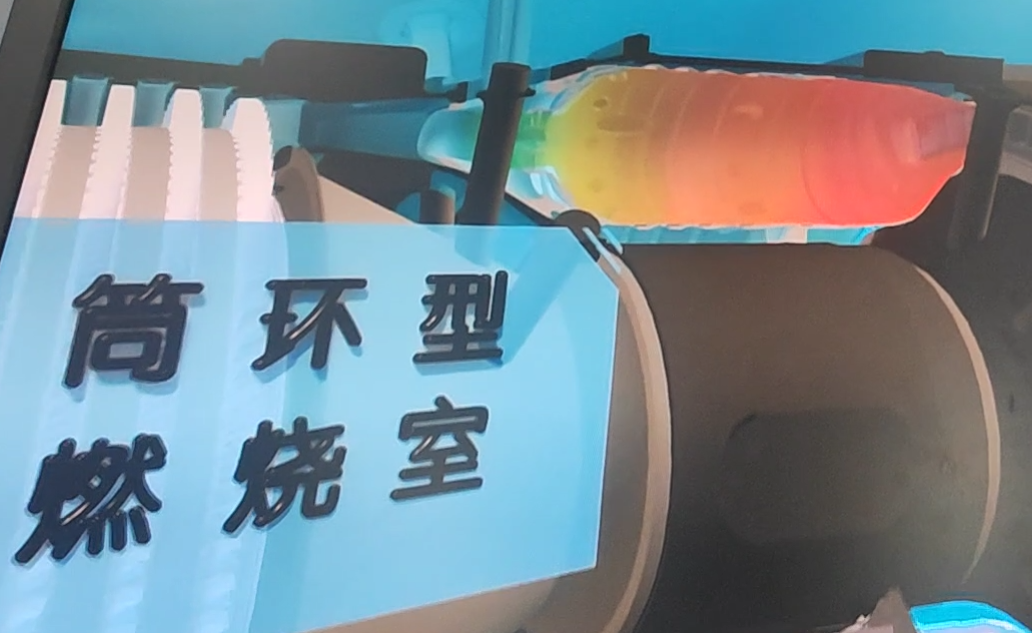
\includegraphics[width=0.85\textwidth]{figures/图6.png}
    \caption{燃烧室结构剖面}
    \label{fig:comb_struct}
\end{figure}

\begin{figure}[H]
    \centering
    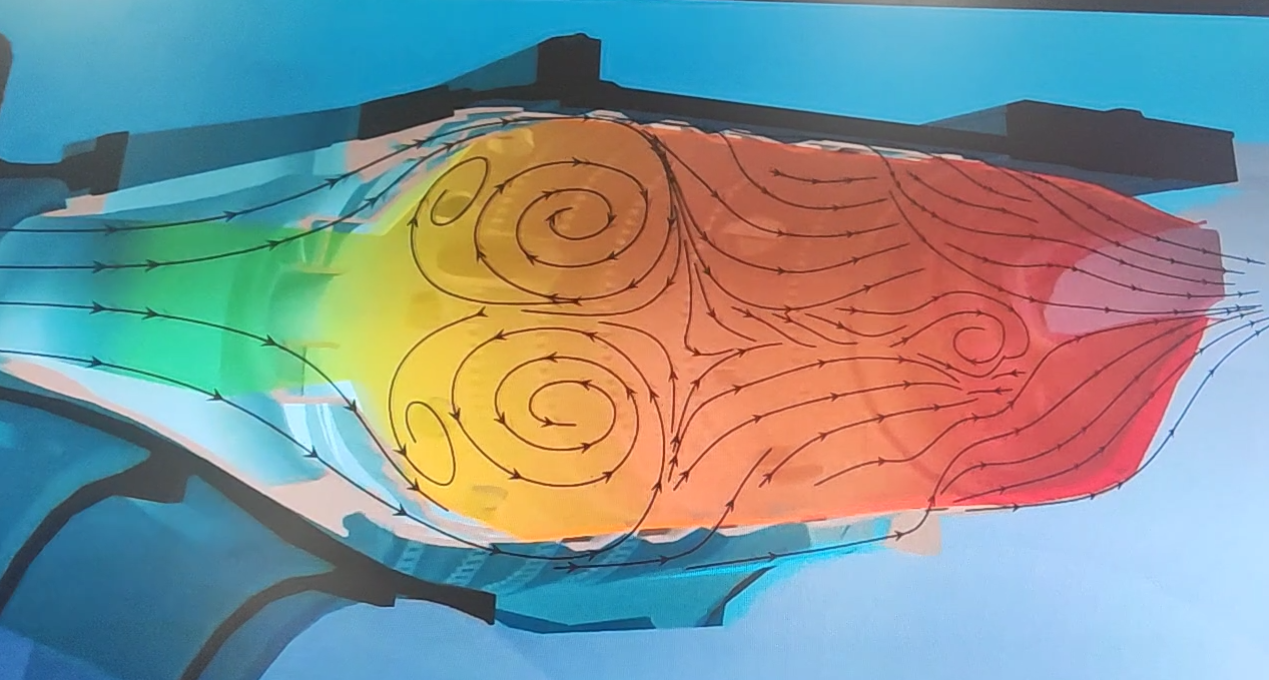
\includegraphics[width=0.90\textwidth]{figures/图7.png}
    \caption{主燃烧室流场——头部双涡回流区}
    \label{fig:comb_flow}
\end{figure}

\textbf{流场拓扑（图~\ref{fig:comb_flow}）：} 通过二维流线切面清晰观察到，主燃区前段形成了对称的双涡回流区。这是由于头部旋流器的强旋流作用所产生的中心驻点反向流动。这个回流区大幅降低了局部气流的轴向速度，使得燃油微滴有充足的时间蒸发并与空气混合，同时将燃烧后的高温燃气带回根部点燃新鲜混气——这是维持核心机连续稳定燃烧的关键气动结构。

\begin{figure}[H]
    \centering
    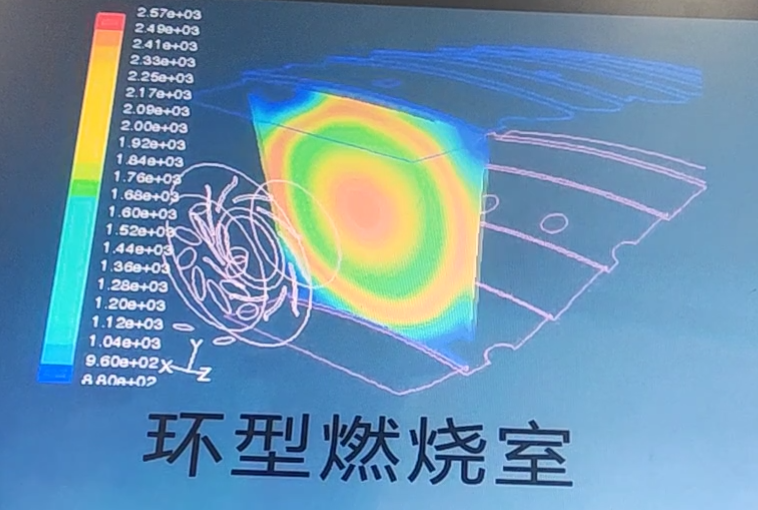
\includegraphics[width=0.90\textwidth]{figures/图8.png}
    \caption{燃烧室温度云图——中心高温区与壁面冷却}
    \label{fig:comb_temp}
\end{figure}

\textbf{温度分布（图~\ref{fig:comb_temp}）：} 温度云图印证了燃烧室截面中心呈现极高的温度梯度。壁面冷却气膜将火焰筒壁面与高温燃气（可达 2000\textasciitilde2400 K）隔离，保证火焰筒结构完整性。

\subsubsection{涡轮流动观察}

\begin{figure}[H]
    \centering
    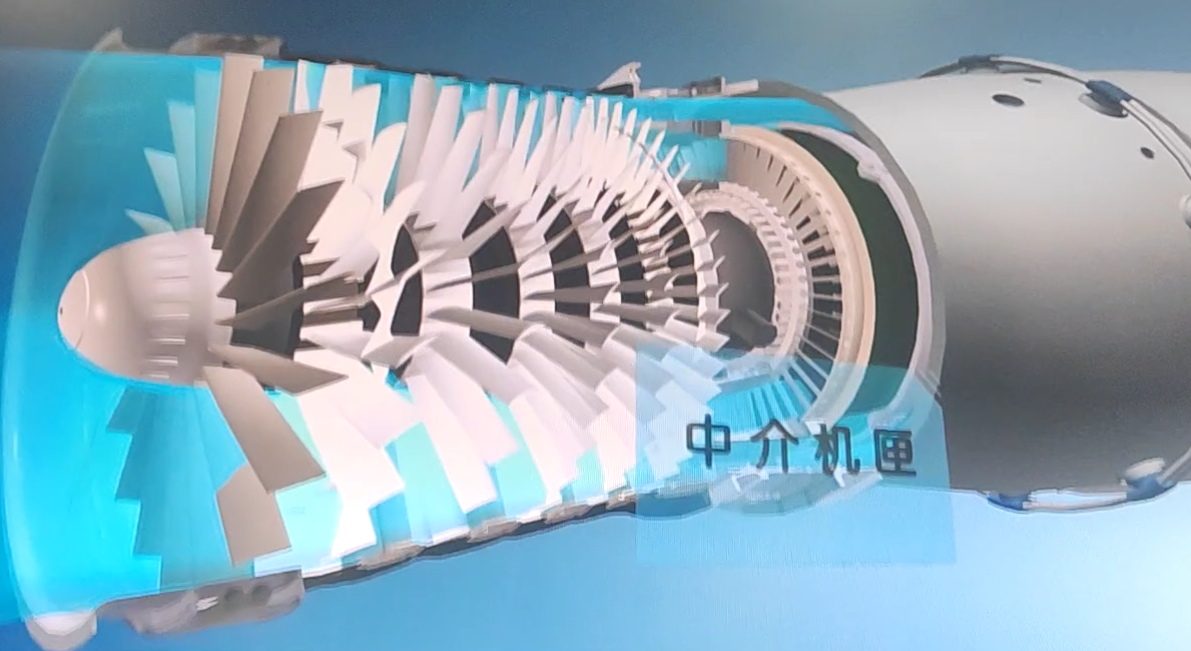
\includegraphics[width=0.85\textwidth]{figures/图1.png}
    \caption{发动机整体结构示意}
    \label{fig:engine_overview}
\end{figure}

\begin{figure}[H]
    \centering
    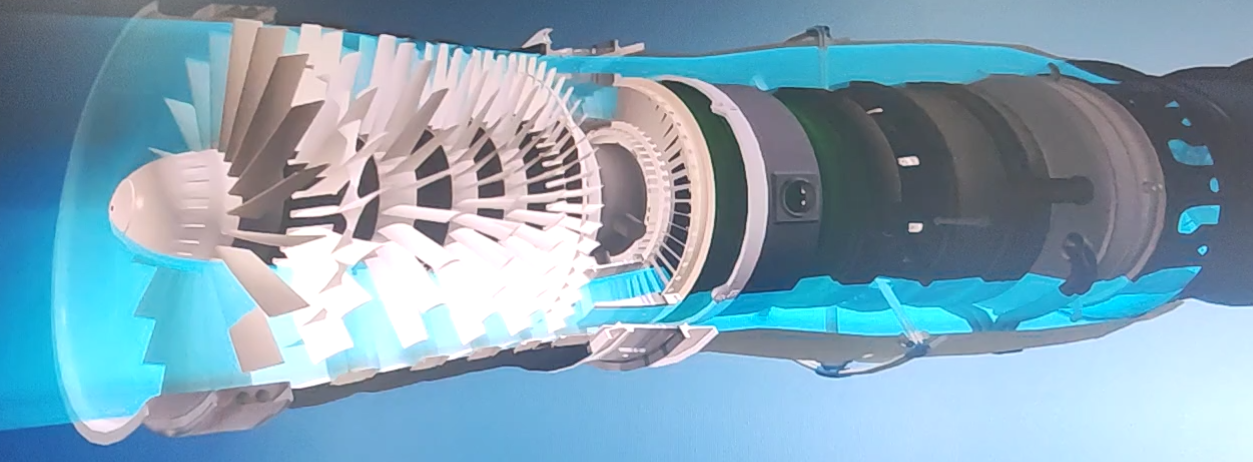
\includegraphics[width=0.85\textwidth]{figures/图2.png}
    \caption{发动机剖面结构}
    \label{fig:engine_section}
\end{figure}

\begin{figure}[H]
    \centering
    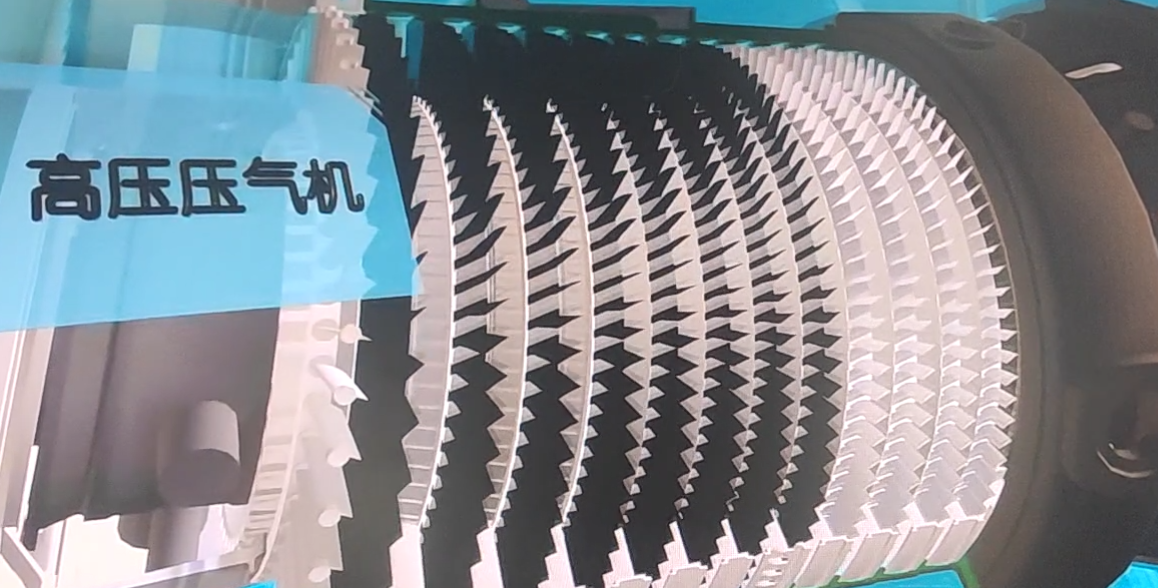
\includegraphics[width=0.85\textwidth]{figures/图3.png}
    \caption{发动机部件示意}
    \label{fig:engine_parts}
\end{figure}

\begin{figure}[H]
    \centering
    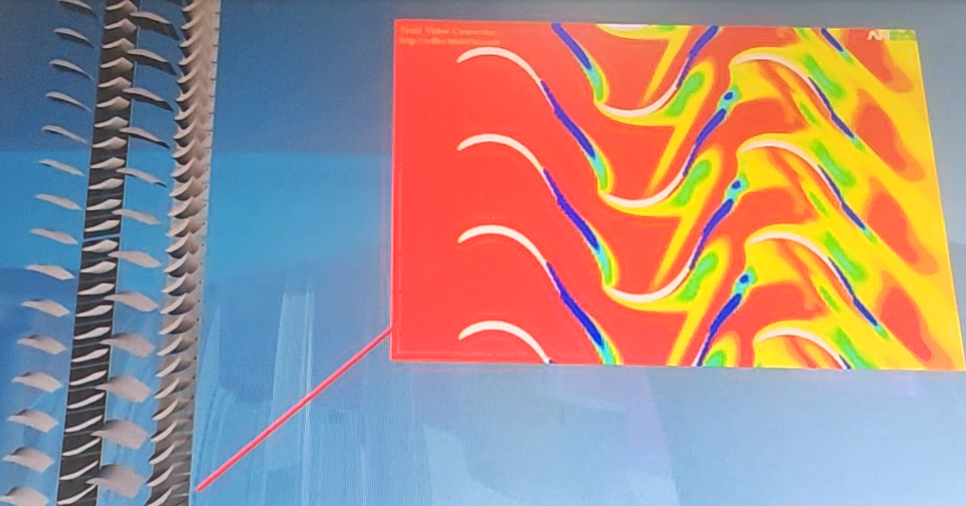
\includegraphics[width=0.90\textwidth]{figures/图9.png}
    \caption{涡轮叶栅流动——渐缩通道内的加速膨胀}
    \label{fig:turbine_flow}
\end{figure}

\textbf{通道几何与流动本质（图~\ref{fig:turbine_flow}）：} 该图展示了高压燃气通过涡轮叶栅时的加速膨胀过程。与压气机叶栅的"渐扩减速增压"通道截然相反，涡轮转子/静子叶片之间构成了明显的渐缩通道（Convergent Passage）。气流在巨大的落压比驱动下，静压能与热能剧烈转化为动能，槽道内的气流表现出极强的压降与加速度。

\textbf{流场云图物理特性：}

\textbf{能量转化梯度：} 图中大面积的红色背景以及向出口方向剧烈的颜色梯度变化，直观地反映了气流马赫数的激增（由低速亚音速膨胀至高亚音速甚至跨声速段），以及静压/静温在轴向上的骤降。

\textbf{局部高载荷区：} 在叶片吸力面的前中部，由于通道收缩和气流转折，气流膨胀速度达到峰值，形成局部的高马赫数区；而压力面相对平缓，这种两侧巨大的流速差形成了驱使涡轮旋转作功的叶片气动力。

\textbf{尾迹与落后角：} 在叶片后缘，可以清晰观察到由于边界层汇聚并脱落形成的狭窄尾迹损失区。若该级为跨声速涡轮，后缘还会伴随有复杂的膨胀波与内剪切激波系，这是阻碍涡轮效率进一步提升的关键流动损失来源。

\subsubsection{排气混合器与加力燃烧室流动观察}

\begin{figure}[H]
    \centering
    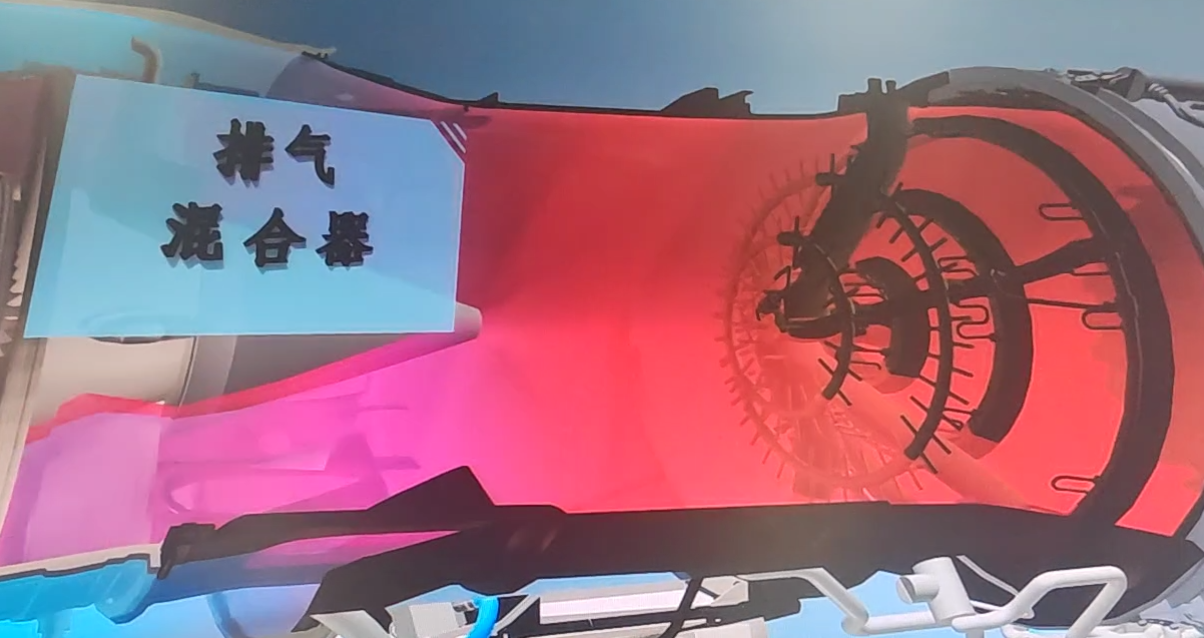
\includegraphics[width=0.90\textwidth]{figures/图10.png}
    \caption{波瓣形排气混合器——冷热气流掺混}
    \label{fig:mixer}
\end{figure}

\textbf{排气混合器（图~\ref{fig:mixer}）：} 展示了典型的波瓣形混合器（Lobed Mixer）结构。通过三维剖面可以观察到，核心机排出的高温燃气（红色区域）与外涵道排出的较低温冷空气在此汇合。波瓣结构极大地扩展了冷热气流的剪切接触面积，并利用几何形状诱导产生强大的流向涡（Streamwise vortices）。这种强迫掺混机制能够有效均匀排气温度场，提升整体推进效率，并显著降低发动机的红外特征和排气噪声。

\begin{figure}[H]
    \centering
    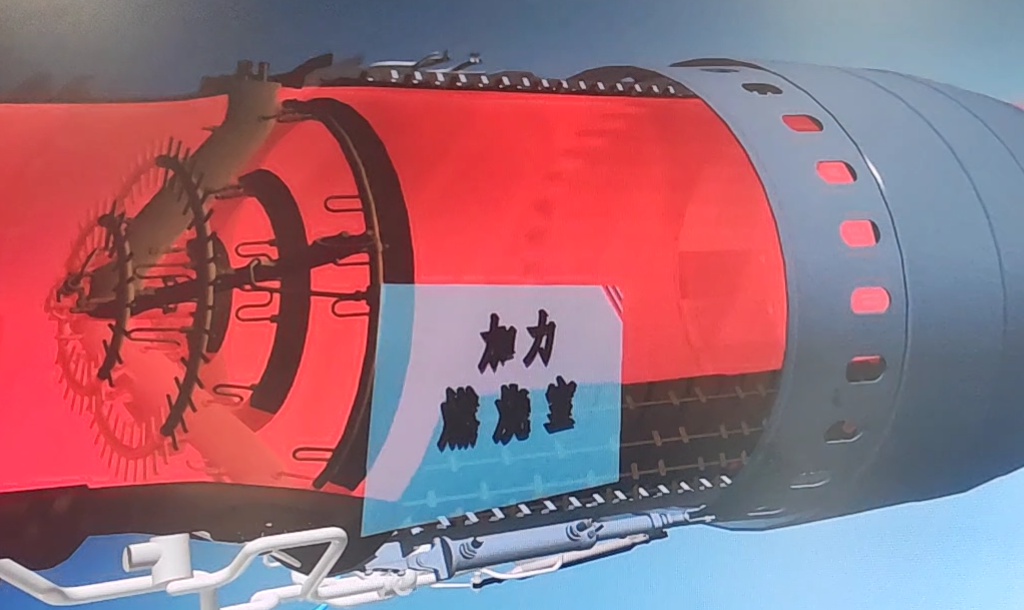
\includegraphics[width=0.90\textwidth]{figures/图11.png}
    \caption{加力燃烧室——火焰稳定器与尾流回流区}
    \label{fig:afterburner_flow}
\end{figure}

\textbf{加力燃烧室（图~\ref{fig:afterburner_flow}）：} 清晰展示了加力燃烧室内部的环形和径向火焰稳定器（V 型钝体/沙丘驻涡器，V-gutter）。在高速流动的排气环境中，气流流经这些非流线型的钝体时，会在其尾缘后方发生边界层分离，形成局部低速的尾流回流区。这一区域起到了"气动避风港"的作用，确保加力时喷入的燃油能够稳定着火，防止火焰被极高流速的主干气流吹熄（Blowout）。

\subsection{实验分析与讨论}

\begin{enumerate}
    \item \textbf{压气机正常流动与失速流动的对比}

    正常工况下，气流沿叶栅通道顺畅流动，附面层紧贴叶片表面，通道内逆压梯度连续均匀，实现了动能向压力能的有效转化。失速工况（如静叶关4°）下，叶片吸力面出现严重的附面层分离，分离区产生巨大的旋涡和回流，形成气动阻塞，通道增压能力丧失。这种由攻角异常增大诱发的分离是发动机喘振的直接原因。

    \item \textbf{燃烧室的稳焰机制与热管理}

    主燃区前段的双涡回流区由旋流器的强旋流作用产生，回流区将高温燃气带回火焰筒头部点燃新鲜混气，是火焰稳定的核心气动结构。温度云图显示截面中心温度梯度极大，壁面冷却气膜对保证火焰筒结构完整性至关重要。

    \item \textbf{排气混合器的波瓣结构}

    波瓣形混合器通过几何形状扩展冷热气流的剪切接触面积，诱导流向涡实现强迫掺混，均匀排气温度场，同时降低红外特征和排气噪声。

    \item \textbf{加力燃烧室的火焰稳定}

    V 型钝体/沙丘驻涡器在高速气流中产生尾流回流区，形成局部低速区使燃油稳定着火，防止被高速主流吹熄。
\end{enumerate}

\subsection{结论}

通过本次虚拟流动实验，结合 CFD 云图和流线可视化结果，对航空发动机四个关键部件的气动热力过程有了深入理解。压气机在设计攻角下流动顺畅而在异常攻角下发生附面层分离引发失速；燃烧室头部双涡回流区实现火焰稳定，壁面冷却气膜保证结构安全；波瓣混合器通过流向涡实现高效掺混；加力燃烧室 V 型钝体后方回流区防止火焰吹熄。实验加深了对《航空发动机原理》和《燃烧学》课程中相关内容的理解。

% !TEX root = ../lab1_report.tex
% ==========================================================
% 实验五：自主探索实验
% ==========================================================
\section{实验五：自主探索实验}

\begin{quote}
\textbf{说明：}该实验允许学生自由发挥，根据个人兴趣自行制定实验方案，方案获审批后方可进行实验。自主探索实验必须具有完整的实验要素。
\end{quote}

\subsection{实验名称}

（根据个人自选课题填写。）

\subsection{实验目的}

（说明本自主探索实验的目的和预期达到的学习目标。建议结合《航空发动机原理》《航空发动机结构》《燃烧学》《叶轮机械原理》等课程所学知识，选择一个感兴趣的切入点进行深入探索。）

\subsection{实验装置}

（列出实验中使用的设备、软件或虚拟系统。可选用的装置包括但不限于：发动机模拟试车系统、三维电子样机、虚拟装配系统、流动显示视频、国家虚拟仿真实验教学平台等。）

\subsection{实验方案}

\subsubsection{实验思路}

（说明选题背景和实验设计思路。建议先进行文献或教材调研，确定探索方向，再设计具体的实验步骤。）

\subsubsection{实验步骤}

\begin{enumerate}
    \item （步骤1）
    \item （步骤2）
    \item （步骤3）
    \item \ldots
\end{enumerate}

\subsection{数据记录}

（记录实验过程中获得的数据，可包含表格、截图等。）

\subsection{数据处理与分析}

（对实验数据进行分析处理，结合理论知识解释实验现象，得出有意义的结论。）

\subsection{结论}

（总结本实验的收获和认识，反思实验设计的不足之处和可能的改进方向。）


\end{document}
